\documentclass[12pt]{article}

\usepackage{amsmath}
\usepackage{array}
\usepackage{caption}
\usepackage[top=1in, bottom=1in, left=0.75in, right=0.75in]{geometry}
\usepackage{graphicx}
\usepackage[colorlinks=true, allcolors=blue]{hyperref}
\usepackage[utf8]{inputenc}
\usepackage{minted}
\usepackage{multirow}
\usepackage{nameref}
\usepackage{pdfpages}
\usepackage[section]{placeins}

\graphicspath{{figures/}}

\begin{document}

\begin{titlepage}
  \begin{center} \LARGE
    \vspace*{1.5in}

    ECE 272 Lab 4

    Fall 2018

    \vfill

    SystemVerilog and Complex Projects

    Phi Luu

    \vfill

    October 31\textsuperscript{st}, 2018

    Grading TA: Edgar Perez

    Lab Partner: Benjamin Geyer

    \vspace{1.5in}
  \end{center}
\end{titlepage}

%%%%%%%%%%%%%%%%%%%%%%%%%%%%%%%%%%%%%%%%%%%%%%%%%%%%%%%%%%%%%%%%%%%%%%%%%%%%%%%%
% Introduction
%%%%%%%%%%%%%%%%%%%%%%%%%%%%%%%%%%%%%%%%%%%%%%%%%%%%%%%%%%%%%%%%%%%%%%%%%%%%%%%%
\section{Introduction}

This lab focuses on implementing combinational logic using a hardware description language (HDL) called SystemVerilog. SystemVerilog uses text to define the specifications of a system. Although it is not as intuitive as describing a system with a schematic (like labs 1, 2, and 3), SystemVerilog allows the users to design more complex systems in a simpler way, especially for sequential circuits.

A simple SystemVerilog-schematic comparison can be seen in a two-input AND gate example in Figure~\ref{figure:1} below:

\begin{figure}[ht]
  \centering
  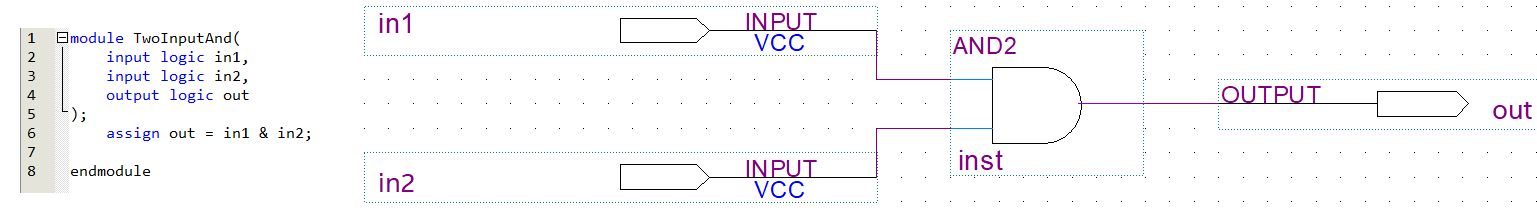
\includegraphics[width=\textwidth]{systemverilog_schematic_comparison.png}
  \caption{A high-accuracy-demand process of drawing a schematic can be simplified into 8 lines of SystemVerilog text file}
  \label{figure:1}
\end{figure}

During this lab, I and Ben design a seven-segment display counter and multiplier. We use 10 switches from the FPGA to represents 10-bit binary numbers, multiply them with a constant according to the input push buttons, and decode the digits to 6 seven-segment displays.

%%%%%%%%%%%%%%%%%%%%%%%%%%%%%%%%%%%%%%%%%%%%%%%%%%%%%%%%%%%%%%%%%%%%%%%%%%%%%%%%
% Design
%%%%%%%%%%%%%%%%%%%%%%%%%%%%%%%%%%%%%%%%%%%%%%%%%%%%%%%%%%%%%%%%%%%%%%%%%%%%%%%%
\section{Design}

We use all 10 switches of the FPGA to represent a 10-bit binary input and 6 seven-segment displays to represent a 6-digit decimal output. To produce the output from the inputs, we implement a 12:17 multiplexer which takes the 10-bit input of the switches as the multiplicand and 2-bit push buttons as the multiplier. The output of the multiplexer is expressed as a 17-bit binary. Next, we parse that output into a parser to split the 17-bit binary into 6 groups of 4-bit binary numbers. Each group of 4-bit binary numbers will then go to a seven-segment display decoder and produce the corresponding digit. Intuitively, the system is illustrated as in Figure~\ref{figure:2} below:

\begin{figure}[ht]
  \centering
  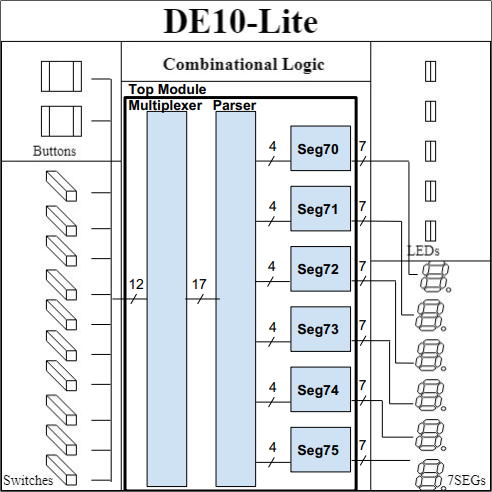
\includegraphics[width=0.6\textwidth]{lab4_block_diagram.png}
  \caption{Block diagram}
  \label{figure:2}
\end{figure}

Since the LEDs in the seven-segment displays are active-low, the output signal needs to be LOW (or $0$) to activate the LEDs and to be HIGH (or $1$) to deactivate the LEDs. Table~\ref{table:1} decodes a decimal number into a binary number and then to the signal in a seven-segment display.

\begin{table}[ht]
  \centering
  \begin{tabular}{ | c | c | c | c | c | c | c | c | c | }
  \hline
  \textbf{Decimal}                                                       & \textbf{Binary}                                                         & \textbf{Seg\textsubscript{A}} & \textbf{Seg\textsubscript{B}} & \textbf{Seg\textsubscript{C}} & \textbf{Seg\textsubscript{D}} & \textbf{Seg\textsubscript{E}} & \textbf{Seg\textsubscript{F}} & \textbf{Seg\textsubscript{G}} \\ \hline
  0                                                                      & 0000                                                                    & 0                             & 0                             & 0                             & 0                             & 0                             & 0                             & 1                             \\ \hline
  1                                                                      & 0001                                                                    & 1                             & 0                             & 0                             & 1                             & 1                             & 1                             & 1                             \\ \hline
  2                                                                      & 0010                                                                    & 0                             & 0                             & 1                             & 0                             & 0                             & 1                             & 0                             \\ \hline
  3                                                                      & 0011                                                                    & 0                             & 0                             & 0                             & 0                             & 1                             & 1                             & 0                             \\ \hline
  4                                                                      & 0100                                                                    & 1                             & 0                             & 0                             & 1                             & 1                             & 0                             & 0                             \\ \hline
  5                                                                      & 0101                                                                    & 0                             & 1                             & 0                             & 0                             & 1                             & 0                             & 0                             \\ \hline
  6                                                                      & 0110                                                                    & 0                             & 1                             & 0                             & 0                             & 0                             & 0                             & 0                             \\ \hline
  7                                                                      & 0111                                                                    & 0                             & 0                             & 0                             & 1                             & 1                             & 1                             & 1                             \\ \hline
  8                                                                      & 1000                                                                    & 0                             & 0                             & 0                             & 0                             & 0                             & 0                             & 0                             \\ \hline
  9                                                                      & 1001                                                                    & 0                             & 0                             & 0                             & 0                             & 1                             & 0                             & 0                             \\ \hline
  \end{tabular}
  \caption{Conversion table between decimal, 4-bit binary, and seven-segment signals}
  \label{table:1}
\end{table}

\newpage

When we implemented a seven-segment display decoder in lab 3, we had to use Karnaugh maps to simplify Boolean equations. We also had to spend a lot of time connecting visual elements on the schematic of Quartus Prime. In this lab, however, we only need to type descriptions of the hardware into SystemVerilog files, and the compiler will take care of the rest. This feature will be quite convenient when we design highly complex circuits in the future.

Because we don't draw any schematic in this lab, we write SystemVerilog code that describes the connections between the elements in the circuit. The source code can be found in the \nameref{section:Appendix} section at the end of this report.

We designate the switch at the corner of the FPGA as bit $0$ of the Switches array in our SystemVerilog code (the switch labeled as \textit{SW0} on the board) and so on. We designate the seven-segment display nearest to the switches as Seg70 (the display labeled \textit{HEX0} on the board). Finally, we designate the push button further from the switches as bit $0$ of the Buttons array in our SystemVerilog code (the button labeled \textit{KEY0} on the board). See the \nameref{section:Appendix} for more details.

%%%%%%%%%%%%%%%%%%%%%%%%%%%%%%%%%%%%%%%%%%%%%%%%%%%%%%%%%%%%%%%%%%%%%%%%%%%%%%%%
% Results
%%%%%%%%%%%%%%%%%%%%%%%%%%%%%%%%%%%%%%%%%%%%%%%%%%%%%%%%%%%%%%%%%%%%%%%%%%%%%%%%
\section{Results}

We compile and simulate the project on ModelSim and obtain the following waveforms:

\begin{figure}[ht]
  \centering
  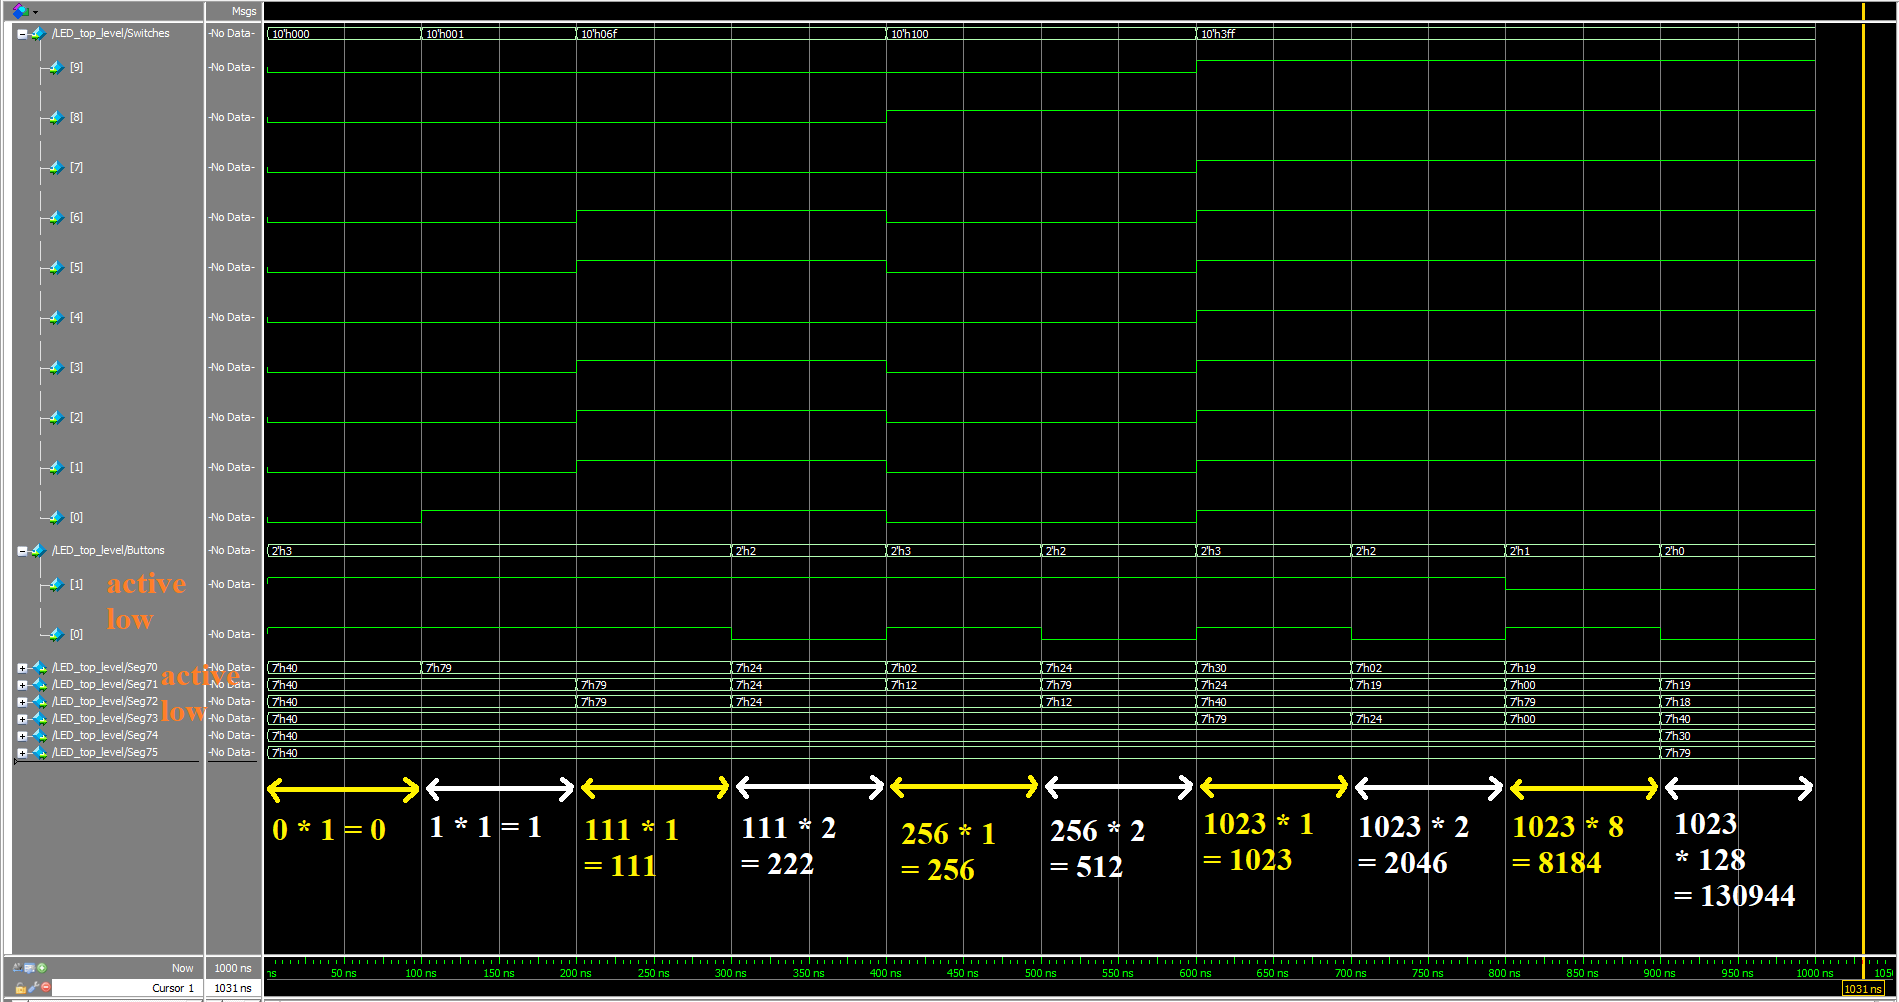
\includegraphics[width=\textwidth]{lab4_simulation.png}
  \caption{Simulation waveform of a few test examples. \href{https://i.imgur.com/1UjCN6E.png}{High-resolution image}}
  \label{figure:3}
\end{figure}

\newpage

Each 100-ns interval (2 columns) is a test case. Each of the test cases' inputs and output are specified with a two-way arrow. For example, from 100 ns to 200 ns (from the third column to the fourth column), the switch input is equivalent to a $1$ in decimal system (\textit{SW1} turned on and all other switches turned off), and the button input is equivalent to a $1$ in decimal system (all buttons not pressed), and the output of all 6 seven-segment display is $000001$ (reading from $\text{Seg75}$ to $\text{Seg70}$).

Using the same method, we obtain the result of all test cases. Since the results are consistent with mathematical calculations, we believe the simulation of the project is a success.

Finally, we upload the project to the real FPGA. We do thorough tests on the real board, and the results are consistent with the simulations as well as mathematical laws. Therefore, we have successfully implemented a seven-segment display decoders with a multiplexer and a parser using SystemVerilog.

%%%%%%%%%%%%%%%%%%%%%%%%%%%%%%%%%%%%%%%%%%%%%%%%%%%%%%%%%%%%%%%%%%%%%%%%%%%%%%%%
% Experiment Notes
%%%%%%%%%%%%%%%%%%%%%%%%%%%%%%%%%%%%%%%%%%%%%%%%%%%%%%%%%%%%%%%%%%%%%%%%%%%%%%%%
\section{Experiment Notes}

%%%%%%%%%%%%%%%%%%%%%%%%%%%%%%%%%%%%%%%%
% Reflection
%%%%%%%%%%%%%%%%%%%%%%%%%%%%%%%%%%%%%%%%
\subsection*{Reflection}

It took me approximately 20 minutes to get used to writing SystemVerilog on Quartus Prime. The combinational logic portion of the project was quite easy. I started to prefer writing SystemVerilog to sketching schematic because I could simplify tedious graphic circuit contruction using a few lines in a \textit{case} block of SystemVerilog.

I think this lab was an easy yet a necessary lab for students to become more familiar with SystemVerilog and how to use HDL to "write" circuits. I plan to program circuits in SystemVerilog from now on because it is more consistent than wiring the components in a graphical interface.

%%%%%%%%%%%%%%%%%%%%%%%%%%%%%%%%%%%%%%%%
% Study Questions
%%%%%%%%%%%%%%%%%%%%%%%%%%%%%%%%%%%%%%%%
\subsection*{Study Questions}

\begin{enumerate}
  \item Describe how to control a 7-seg display using a state machine and lighting each digit one at a time.

  Let each state be a seven-segment display of the array of 6 displays on the FPGA, so there are six separate states: S0 corresponding to Seg70, S1 corresponding to Seg71, S2 corresponding to Seg72, S3 corresponding to Seg73, S4 corresponding to Seg74, and S5 corresponding to Seg75.

  The inputs are the switches and the push buttons.
\end{enumerate}

%%%%%%%%%%%%%%%%%%%%%%%%%%%%%%%%%%%%%%%%%%%%%%%%%%%%%%%%%%%%%%%%%%%%%%%%%%%%%%%%
% Appendix
%%%%%%%%%%%%%%%%%%%%%%%%%%%%%%%%%%%%%%%%%%%%%%%%%%%%%%%%%%%%%%%%%%%%%%%%%%%%%%%%
\section*{Appendix} \label{section:Appendix}

\begin{center}
  \textbf{lab4.qsf} (Pin Assignment)
\end{center}

\begin{minted}[linenos]{text}
set_location_assignment PIN_C14 -to Seg70[0]
set_location_assignment PIN_E15 -to Seg70[1]
set_location_assignment PIN_C15 -to Seg70[2]
set_location_assignment PIN_C16 -to Seg70[3]
set_location_assignment PIN_E16 -to Seg70[4]
set_location_assignment PIN_D17 -to Seg70[5]
set_location_assignment PIN_C17 -to Seg70[6]
set_location_assignment PIN_C18 -to Seg71[0]
set_location_assignment PIN_D18 -to Seg71[1]
set_location_assignment PIN_E18 -to Seg71[2]
set_location_assignment PIN_B16 -to Seg71[3]
set_location_assignment PIN_A17 -to Seg71[4]
set_location_assignment PIN_A18 -to Seg71[5]
set_location_assignment PIN_B17 -to Seg71[6]
set_location_assignment PIN_B20 -to Seg72[0]
set_location_assignment PIN_A20 -to Seg72[1]
set_location_assignment PIN_B19 -to Seg72[2]
set_location_assignment PIN_A21 -to Seg72[3]
set_location_assignment PIN_B21 -to Seg72[4]
set_location_assignment PIN_C22 -to Seg72[5]
set_location_assignment PIN_B22 -to Seg72[6]
set_location_assignment PIN_F21 -to Seg73[0]
set_location_assignment PIN_E22 -to Seg73[1]
set_location_assignment PIN_E21 -to Seg73[2]
set_location_assignment PIN_C19 -to Seg73[3]
set_location_assignment PIN_C20 -to Seg73[4]
set_location_assignment PIN_D19 -to Seg73[5]
set_location_assignment PIN_E17 -to Seg73[6]
set_location_assignment PIN_F18 -to Seg74[0]
set_location_assignment PIN_E20 -to Seg74[1]
set_location_assignment PIN_E19 -to Seg74[2]
set_location_assignment PIN_J18 -to Seg74[3]
set_location_assignment PIN_H19 -to Seg74[4]
set_location_assignment PIN_F19 -to Seg74[5]
set_location_assignment PIN_F20 -to Seg74[6]
set_location_assignment PIN_J20 -to Seg75[0]
set_location_assignment PIN_K20 -to Seg75[1]
set_location_assignment PIN_L18 -to Seg75[2]
set_location_assignment PIN_N18 -to Seg75[3]
set_location_assignment PIN_M20 -to Seg75[4]
set_location_assignment PIN_N19 -to Seg75[5]
set_location_assignment PIN_N20 -to Seg75[6]
\end{minted}

\begin{center}
  \textbf{LED\_top\_level.sv}
\end{center}

\begin{minted}[linenos]{systemverilog}
module LED_top_level(
    input logic [9:0] Switches,
    input logic [1:0] Buttons,
    output logic [6:0] Seg70, Seg71, Seg72, Seg73, Seg74, Seg75
);
    /*******************************/
    /* Set internal variables here */
    /*******************************/
    logic [16:0] m_out;
    logic [3:0] p_out0, p_out1, p_out2, p_out3, p_out4, p_out5;

    /********************************************/
    /* Instanciate and Connect all modules here */
    /********************************************/

    Multiplexer M(
        .switches(Switches),
        .buttons(Buttons),
        .out(m_out)
    );

    Parser P(
        .in(m_out),
        .out0(p_out0),
        .out1(p_out1),
        .out2(p_out2),
        .out3(p_out3),
        .out4(p_out4),
        .out5(p_out5)
    );

    Decoder D0(
        .Num(p_out0),
        .segments(Seg70)
    );
    Decoder D1(
        .Num(p_out1),
        .segments(Seg71)
    );
    Decoder D2(
        .Num(p_out2),
        .segments(Seg72)
    );
    Decoder D3(
        .Num(p_out3),
        .segments(Seg73)
    );
    Decoder D4(
        .Num(p_out4),
        .segments(Seg74)
    );
    Decoder D5(
        .Num(p_out5),
        .segments(Seg75)
    );

endmodule
\end{minted}

\begin{center}
  \textbf{Multiplexer.sv}
\end{center}

\begin{minted}[linenos]{systemverilog}
module Multiplexer(
    input logic [9:0] switches,
    input logic [1:0] buttons,
    output logic [16:0] out
);

    always_comb
        case(buttons)
            0: out = switches * 128;
            1: out = switches * 8;
            2: out = switches * 2;
            3: out = switches;
        endcase

endmodule
\end{minted}

\begin{center}
  \textbf{Parser.sv}
\end{center}

\begin{minted}[linenos]{systemverilog}
module Parser(
    input logic [16:0] in,
    output logic [3:0] out0, out1, out2, out3, out4, out5
);

    always_comb begin
        out0 = in % 10;
        out1 = (in / 10) % 10;
        out2 = (in / 100) % 10;
        out3 = (in / 1000) % 10;
        out4 = (in / 10000) % 10;
        out5 = (in / 100000) % 10;
    end

endmodule
\end{minted}

\begin{center}
  \textbf{Decoder.sv}
\end{center}

\begin{minted}[linenos]{systemverilog}
module Decoder(
    input logic [3:0] Num,
    output logic [6:0] segments
);
    always_ff @(*)
        case(Num)
            0: segments=7'b100_0_000;
            1: segments=7'b111_1_001;
            2: segments=7'b010_0_100;
            3: segments=7'b011_0_000;
            4: segments=7'b001_1_001;
            5: segments=7'b001_0_010;
            6: segments=7'b000_0_010;
            7: segments=7'b111_1_000;
            8: segments=7'b000_0_000;
            9: segments=7'b001_1_000;
            default: segments= 7'b111_1111;
        endcase

endmodule
\end{minted}

\end{document}
